Para la interfaz de usuario, cabe aclarar que se usó en la mayoría de las interfaces una filosofía específica para que el usuario utilizara las funcionalidades ofrecidas por el SNS deportivo: La idea de tener dos botones que abren dos menús (uno a la izquierda, otro a la derecha) los cuales, respectivamente, indican funcionalidades generales y funcionalidades específicas. Un ejemplo se consigna en las figuras \ref{fig:ui_ejemplo_1} y \ref{fig:ui_ejemplo_2}:

\begin{figure}[!htb]
  \begin{center}
    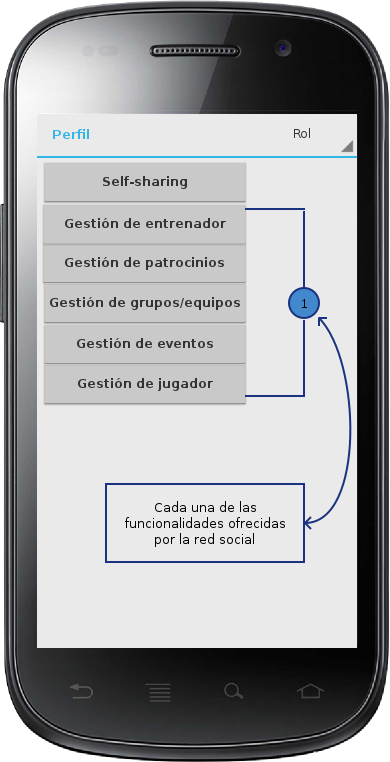
\includegraphics[width=7cm]{./imagenes/UI/Self_sharing/self_sharing_1.png}
    \caption{Menú izquierdo correspondiente a funcionalidades más generales}
    \label{fig:ui_ejemplo_1}
    \textbf{Fuente:}  Autores
  \end{center}
\end{figure}

Se ve en el menú izquierdo que se incluyen todas las funcionalidades que el SNS completo debería prestar.

\begin{figure}[!htb]
  \begin{center}
    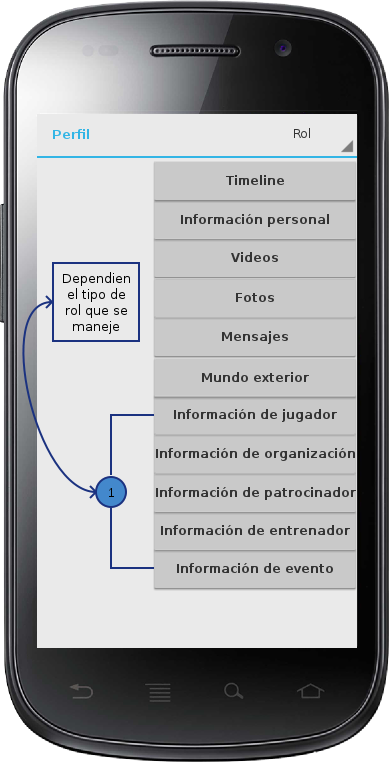
\includegraphics[width=7cm]{./imagenes/UI/Self_sharing/self_sharing_2.png}
    \caption{Menú derecho correspondiente a funcionalidades más específicas}
    \label{fig:ui_ejemplo_2}
    \textbf{Fuente:}  Autores
  \end{center}
\end{figure}

Se ve en el menú derecho que se incluyen funcionalidades específicas al módulo de gestión de self-sharing, por lo que el usuario debió haber elegido del menú izquierdo la funcionalidad específica de gestión de self-sharing.

El panel de la izquierda será activado por medio del botón menú que traen los dispositivos android. Por su parte, el menú de la derecha aparecerá al usar el botón que se ha nombrado en los bosquejos "Acción", por convención y comodidad.

Para saber más acerca del prototipo creado para la interfaz, el lector puede consultar en \ref{app:ui} para ver más detalladamente todas las vistas creadas.